\section {ECN versus Delay}
\label{sec:discuss}
In the previous sections, we saw that barring the small anomaly, DCQCN remains
stable as the number of flows increase. We also saw that this is not the case
for TIMELY. However, for both protocols, the fixed point of the queue
and hence the round trip delay increases with the number of contending
flows, and this makes designing the controller more difficuly with TIMELY as compared to DCQCN.


Let's assume a single-bottleneck scenario, and assume that ECN marking is used
to convey congestion information. Typical shared-buffer switches, especially
those that use Broadcom's merchent sillicon, do ECN marking on {\em packet
egress}. When a packet is ready to depart, the controller checks the egress
queue for that port {\em at that instant}, and depending on the specified
marking algorithm (e.g.  Equation~\ref{eq:mark}), decides whether to mark the
packet. Thus, the mark carried by the packet conveys information about the state
of the queue at the time the packet {\em departs} the queue. In other words,
information carried by just-departed packet (say $p_i$) is influenced by all the
packets that arrived in the queue {\em after} $p_i$ arrived, but before $p_i$
left. 

On the other hand, consider what RTT measurements do. If the egress queue
discipline is FIFO within a priority class, (which it typically is), the delay
experienced by a packet reflects the state of the queue at the time the packet
{\em arrives} at the queue. Subsequent packet arrivals have no bearing on the
delay experienced by the packet. 

This seemingly small detail means that the information about queue state
conveyed by RTT measurements is always {\em stale} compared to what can be
conveyed by ECN markings. In practice, this means that as the queue length
increases, congestion control algorithms that rely on RTT suffer from increasing
{\em lag} in their control loop, making them unstable. Since steady state queue
length typically increases with number of flows, RTT based congestion control is
is more likely to become unstable, compared to ECN-based congestion control.

This issue is critical in data center networks, because queueing delays can
easily dominate switching and propagation delays.  For example, an Arista
7040QX32 has 40Gbps ports, and a total shared buffer of switch has 12MB. Even if
just 1MB worth of queue builds ip at an egress port, it takes 200 $\mu$s to
drain. In contrast, the one-hop propagation delay, with cut-through forwarding
is enabled, are in the range of 1-2 $\mu$s. Typical diameter of a DC network is
6 hops, propagation delay is just 10-18 $\mu$s. In contrast, in wide area
networks, queuing delays and propagation delays can be comparable (excluding
scenarios like buffer bloat~\cite{bufferbloat}). 

However, one can ask the question - can we build congestion control protocols
that are guaranteed to maintain a fixed queue length at the bottleneck,
regardless of the number of flows? The answer, as we show below, turns out to be
yes - but you can guarantee fairness only if you use ECN.

The key to building protocols that guarantee delay to a fixed quantity
is to use a controller with \emph{integral} control. In the context of
network transport protocols and AQM, integral control was first introduced
by the PI controller~\cite{hollot2001designing}\footnote{ 
The PI controller has also been used to solve the problem of bufferbloat~\cite{conf/hpsr/PanNPPSBV13,bufferbloat-pi}~, and
has become part of the DOCSIS 3.1 standard}~and
REM~\cite{REM}.
The idea behind integral control is to look at an
error signal, e.g. the difference between the actual queue length and
a desired or reference queue length, and adjust the feedback until the
error signal goes to 0 and a stable PI controller is guaranteed to
achieve that. In a continuous system, the feedback signal $p(t)$
evolves in the following way with a PI controller:

$$ \frac{dp}{dt} = K_1\frac{de}{dt}+K_2e(t) $$

When the feedback signal converges, both the error signal $e(t)$ as
well as the derivative of the error signal, $de/dt$ must converge to
0. The derivative of the error signal, (the derivative of the queue length), goes to 0
when the sum of the rates $R_i$ match the link capacity $C$. The error signal itself goes to 0
when the queue length matches the reference value. Thus the integral
controller implements the ``match rate, clear buffer'' scheme
presented in~\cite{REM}. For DCQCN we can implement the PI
controller to mark the packets at the switch instead of RED (which is
a proportional controller without the integral action) and use that
$p$ in the usual way to perform the multiplicative decrease. For
(patched) TIMELY, we can
measure the delay at the end hosts and implement a PI controller by
generating an internal variable ``p'', using the error signal
``$e(t)$'' as the difference between the measured delay and some
reference or desired delay. This internal variable $p$ can then
replace the $\tfrac{{q(t - \tau ') - q'}}{{q'}}$ term in
Equation (\ref{eq:timely_fixed}) as the feedback to control the rates.

We implemented the PI controller for both the DCQCN and patched TIMELY
fluid models and performed simulations. As we see in
Figure~\ref{fig:dcqcn_pi}~for DCQCN, the queue length is stabilized to a
preconfigured value, regardless of the number of flows (as well as
regardless of propagation delay). This is important not only for
stability, but also for performance reasons in a datacenter network.

\begin{figure}
\subfigure[] {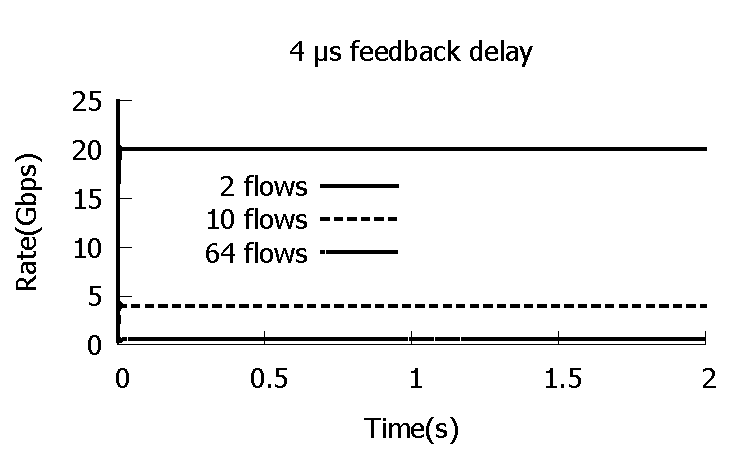
\includegraphics[width=0.49\columnwidth]{figures/stable_rate_4_pifixed.pdf}}
\subfigure[] {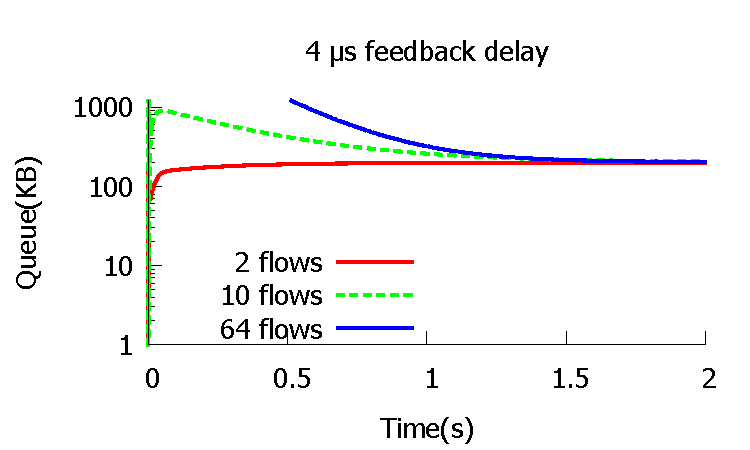
\includegraphics[width=0.49\columnwidth]{figures/stable_q_4_pifixed.pdf}}
\caption{DCQCN with PI controller}
\label{fig:dcqcn_pi}
\end{figure}

In contrast, when we use a PI controller at the end hosts with patched
TIMELY, we see that although we can control the queue
to a specified value (300 KB), we cannot achieve fairness. Thus, while
patched TIMELY was able to achieve fairness without guaranteeing
delay, patched TIMELY with PI is able to guarantee delay without
achieving fairness.
\begin{figure}
\center
\subfigure[Two flows (7 and 3Gbps)]
{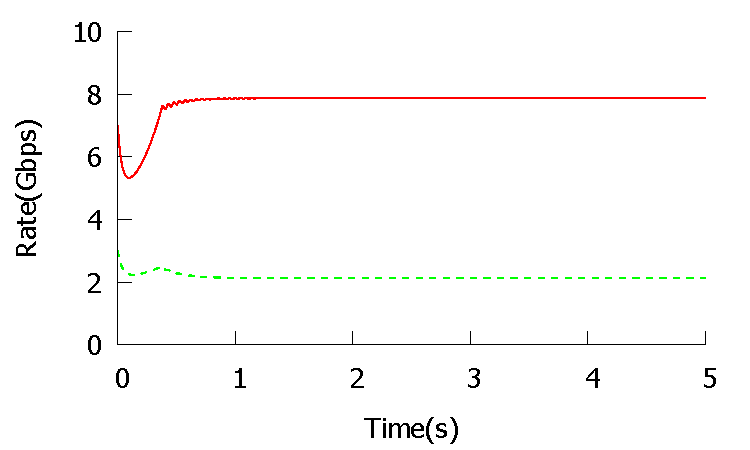
\includegraphics[width=0.49\columnwidth]{figures/timely_withpi_2_4_rate.pdf}}
\subfigure[Two flows (7 and 3Gbps)] {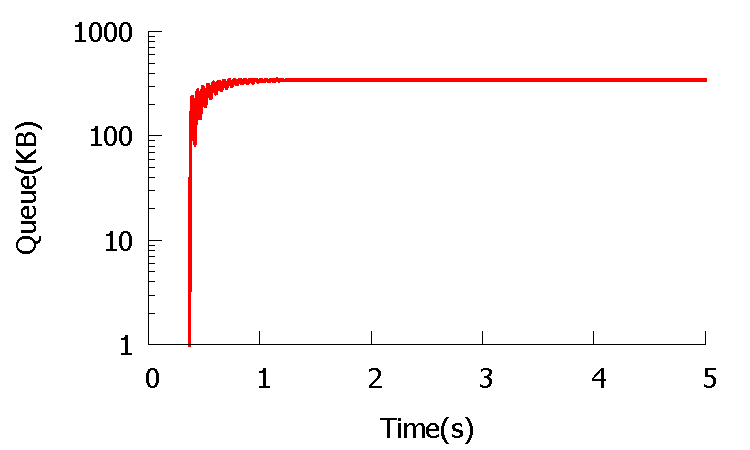
\includegraphics[width=0.49\columnwidth]{figures/timely_withpi_2_4_queue.pdf}}
\subfigure[Ten flows] {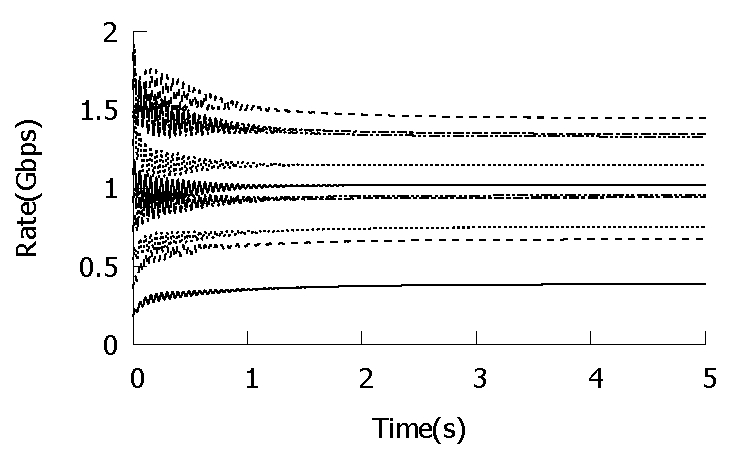
\includegraphics[width=0.49\columnwidth]{figures/timely_withpi_10_4_rate.pdf}}
\subfigure[Ten flows] {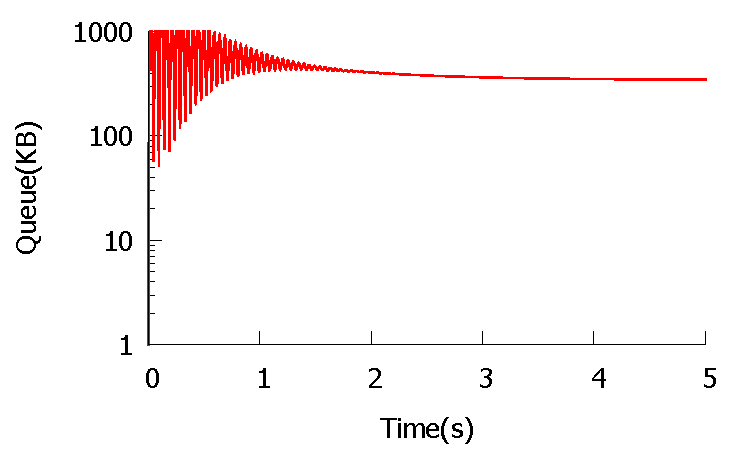
\includegraphics[width=0.49\columnwidth]{figures/timely_withpit_10_4_queue.pdf}}
\caption{PI controller to stabilize TIMELY}
\label{fig:timely_pi}
\end{figure}

We next prove a result that formalizes this fundamental tradeoff between fairness
and guaranteed delay for protocols that rely on delay measurements at the end
points to implement congestion control.

\begin{thm}[Fairness/Delay tradeoff]
\label{thm:fairness-delay}
For congestion control mechanisms that relay purely on end to end
delay measurements, you can either have fairness or a guaranteed delay
bound, but not both simultaneously.
\end{thm}
\begin{proof}
Suppose you have N flows sharing a link of capacity $C$. Then every flow
should distributedly arrive at a rate $C/N$ and the flows need to know
this $N$. If we use end to end delay as the only signal, then this delay
has to carry information about $N$ and hence the converged delay
depends on $N$ and cannot be guaranteed independently. Conversely, if we implement a guaranteed delay congestion
control scheme at the end points, they
will converge to any rate $R_i$ such that $\sum_{i=0}^{N}R_i = C$
making the derivative of measured delay 0 and the actual delay equal
to the guarantee. Since the guarantee is set independent of $N$, the
actual delay contains no information on N and 
thus such a scheme cannot ensure fairness.
\end{proof}

\noindent
Based on these two factors, the faster feedback to the sources as well
as the ability to simultaneously achieve fairness and bounded delay
point strongly in favor of using ECN instead of delay in a datacenter
environment for congestion control. Even though using delay as a
feedback signal has a simpler
implementation path not requiring switch support, delay based
congestion control has fundamental limitations. Note that TCP, or more
precisely AIMD, is also an end system based congestion control
mechanism but it uses loss probability as the feedback signal. This
loss probability depends upon the number of flows and hence that
information is encoded in the feedback and so it does not suffer from
the same limitation. 

A full exploration of PI (like)
controllers for RDMA including a hardware implementation is under
active study by us and is beyond the scope of this paper.
%%% Local Variables:
%%% mode: latex
%%% TeX-master: "main"
%%% End:
